\chapter{Modificación de la Fuente CC anterior}
% ----------------------

\label{C:Sobre la fuente anterior}

\section{Fuente de alimentación CC lineal a modificar}
La revisión y adaptación del trabajo previo titulado \entreComillas{Diseño y construcción de una fuente de alimentación CC lineal con control digital de tensión y corriente} llevado a cabo por Eduardo Javier Matijak y Joaquín Pelinski, documentado en su publicación \cite{Fuente2023}, sirve como punto de partida para comprender las mejoras implementadas en la fuente de alimentación DC que se examina en este informe. \textbf{Invitamos cordialmente al lector interesado a consultar dicho trabajo para obtener una comprensión más completa de los fundamentos sobre los cuales se basa este análisis.} \par 
Esta sección se centra en analizar y discutir las modificaciones realizadas en la fuente de alimentación, específicamente la transición de su mayoría analógica a una configuración digital. Entre los principales cambios introducidos se destacan los siguientes aspectos:

\subsection{Circuito Fijador de Referencia para los Transistores}
El circuito fijador de referencia para los transistores ha sido modificado para incorporar la salida de un Convertidor Analógico-Digital (DAC). El DAC es ahora responsable de aplicar niveles de voltaje acorde a los valores determinados por el control digital. Esta modificación permite un ajuste preciso y programable de las referencias de voltaje, eliminando la necesidad de ajustes mecánicos, por ende mejorando la precisión y flexibilidad del sistema.
\begin{figure}[H]
    \centering
    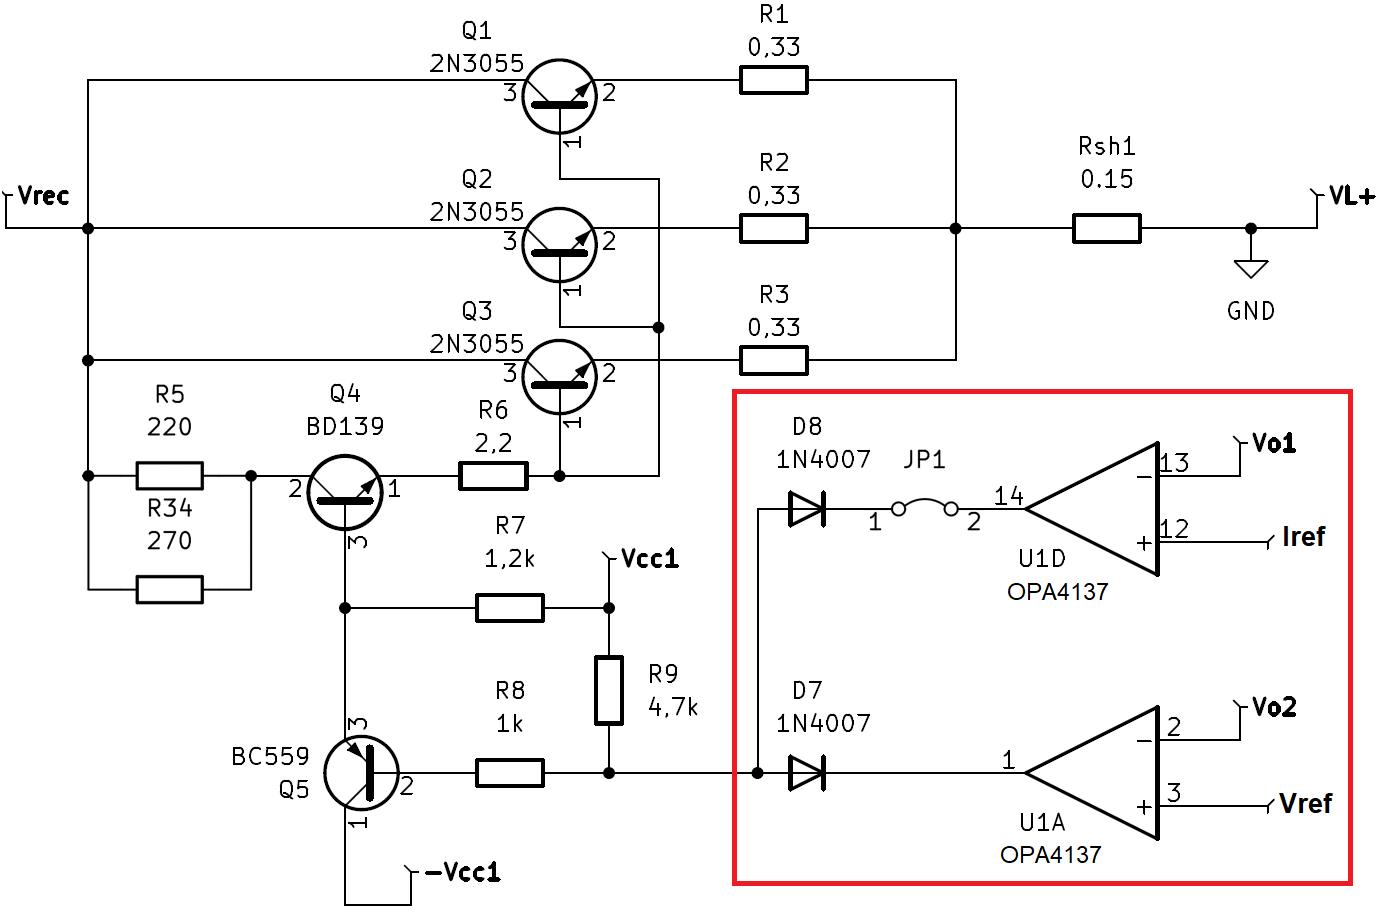
\includegraphics[width=0.8\textwidth]{./imagenes/Eliminada1.PNG}
    \caption{Sección de referencia de tensión a aplicar sobre la base de los transistores.}
    \label{F:Eliminada1}
\end{figure}\par 
Entre los cambios a realizarse a la Figura \ref{F:Eliminada1} se incluye la sustitución de la resistencia de \textit{pull-up} R9 por una de \textit{pull-down}. Se agrega además un seguidor de tensión del voltaje de salida del DAC que inyecte la misma magnitud sobre la base del transistor Q5.

\subsection{Modificación de uso de Potenciómetros Digitales MCP4661}
Originalmente, los potenciómetros digitales MCP4661 se utilizaban para establecer una referencia de voltaje que comandaba los transistores, definiendo tanto la tensión como la corriente sobre la carga. Sin embargo, con la incorporación del DAC, esta función ya no es necesaria. En su lugar, los potenciómetros digitales ahora se utilizan para establecer una referencia de tensión destinada a un circuito de protección analógica contra cortocircuitos. Esta reasignación permite una respuesta inmediata para proteger la carga, evitando los retrasos inherentes a los cálculos y actualizaciones de salida necesarios en un sistema de control digital.
\begin{figure}[H]
    \centering
    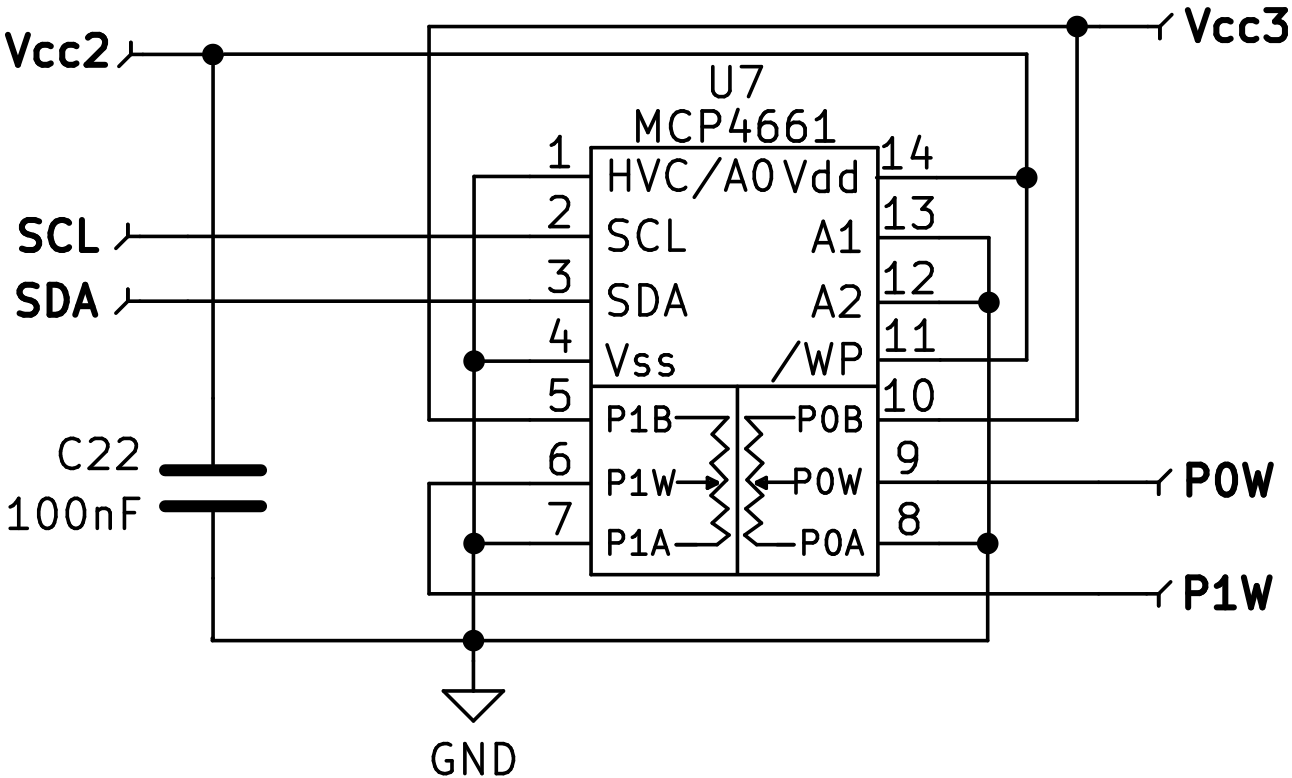
\includegraphics[width=0.5\textwidth]{./imagenes/potenciometro_digital.png}
    \caption{Símbolo del potenciómetro digital MCP4661.}
    \label{F:potenciometro_digital}
\end{figure}
En la Figura \ref{F:potenciometro_digital} podemos observar el símbolo del potenciómetro mencionado. Con el mismo es posible modificar el porcentaje de resistencia mediante comunicación digital a través del protocolo \entreComillas{Circuito Inter-Integrado} (I2C).

\subsection{Eliminación del circuito de medición externo}
Dado que la fuente de alimentación ahora cuenta con una pantalla integrada que muestra en tiempo real los valores de tensión y corriente, el circuito dedicado a la conexión de un voltímetro-amperímetro digital se ha considerado innecesario y, por lo tanto, ha sido removido del diseño. Esta simplificación reduce la complejidad y el número de componentes necesarios reduciendo los costos constructivos de la fuente.
\begin{figure}[H]
    \centering
    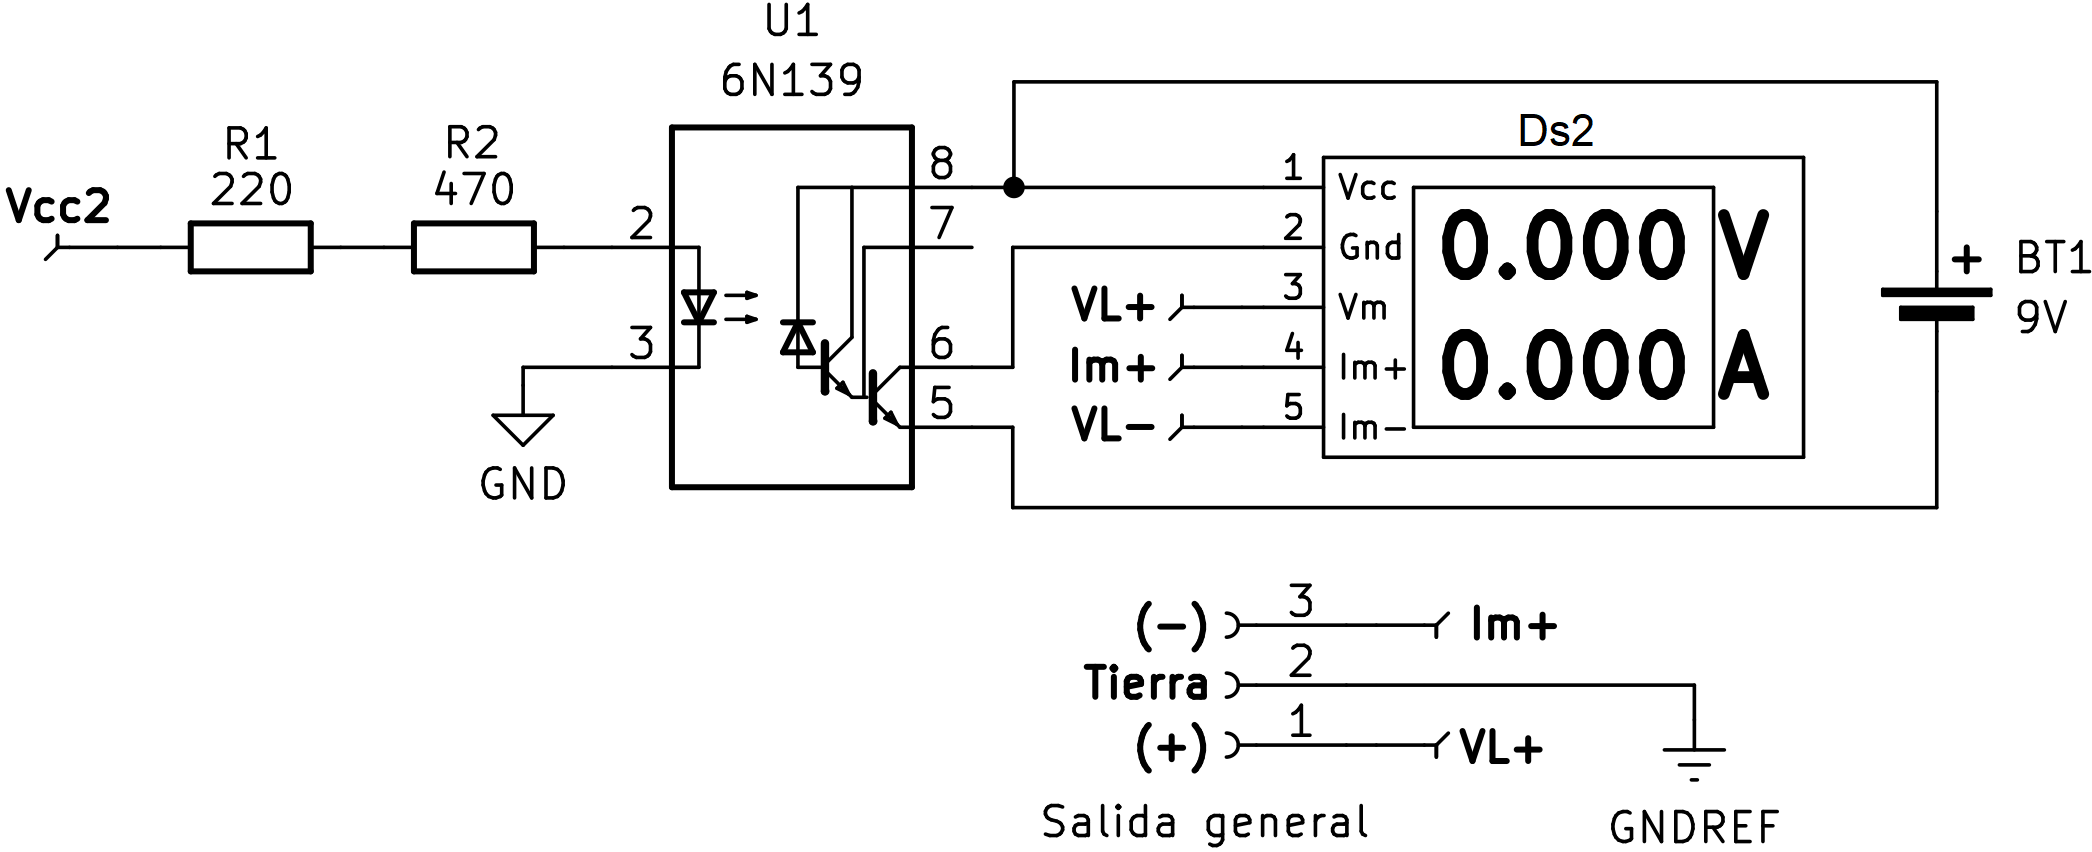
\includegraphics[width=0.8\textwidth]{./imagenes/voltimetro_amperimetro.png}
    \caption{Conexión voltímetro/amperímetro.}
    \label{F:voltimetro_amperimetro}
\end{figure}
En la Figura \ref{F:voltimetro_amperimetro} se aprecia los interconexión de los elementos que conformaban esta etapa. También se resalta que para su correcto funcionamiento era necesario una batería de 9V.

\subsection{Modificación del Circuito de Acople y Desacople de Carga}\par 
Se ha modificado considerablemente el circuito de disparo del relé de acople y desacople de carga, aprovechando las capacidades proporcionadas por el \entreComillas{Arduino Nano} con sus entradas y salidas digitales.
\begin{figure}[H]
    \centering
    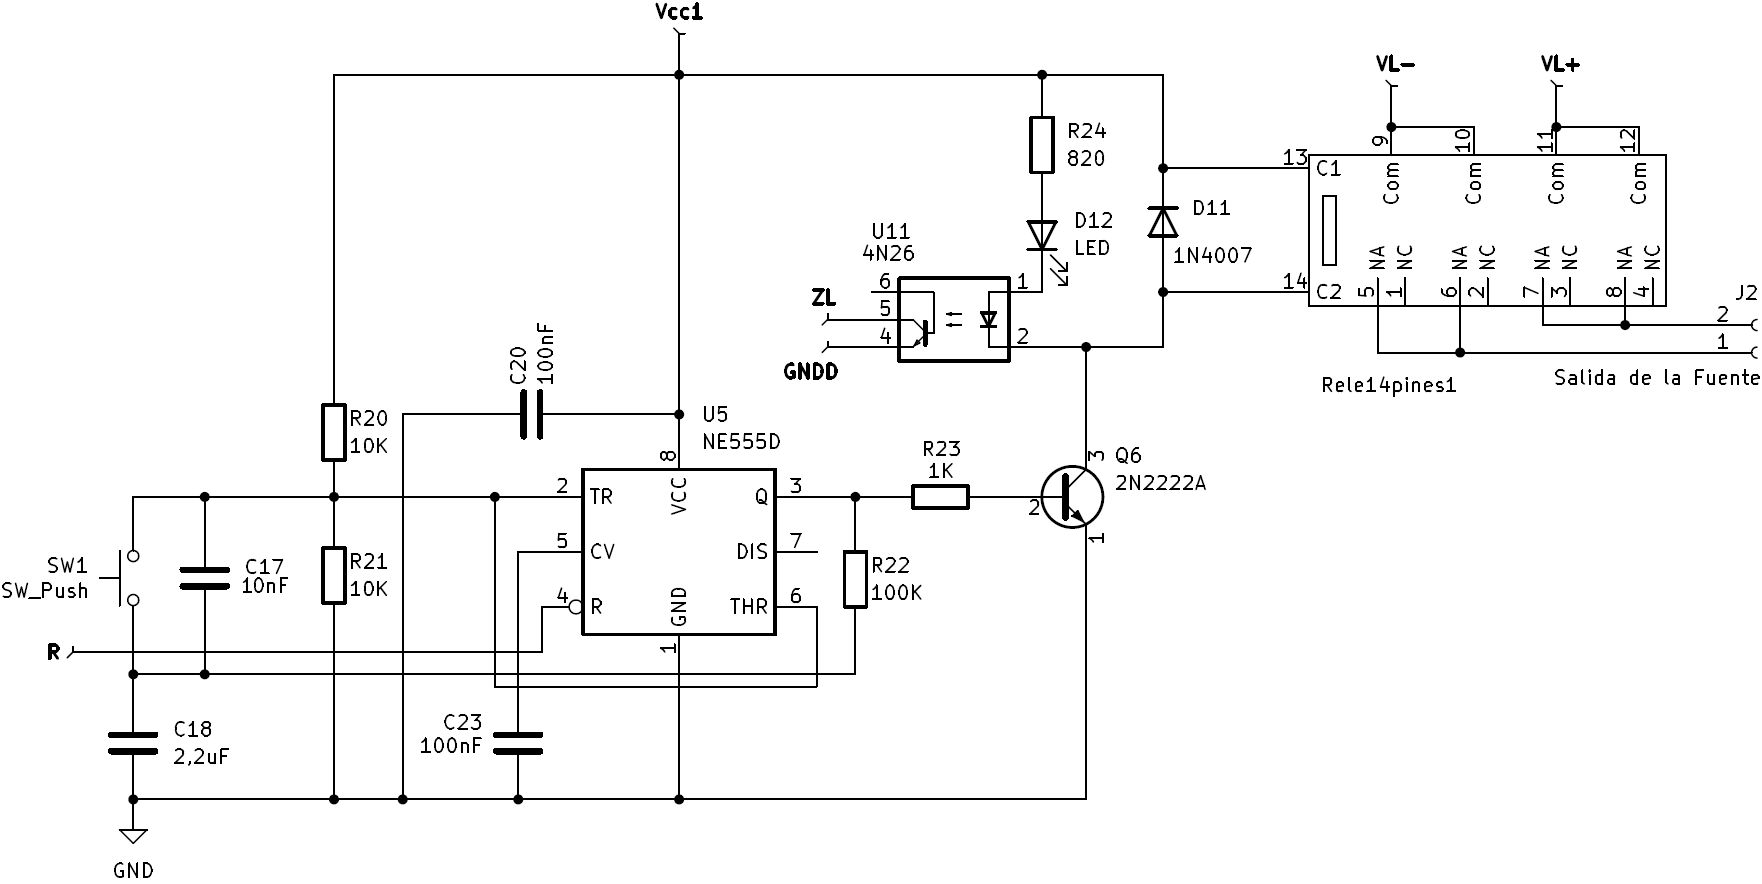
\includegraphics[width=0.9\textwidth]{./imagenes/conexion_carga.PNG}
    \caption{Acople y desacople de carga.}
    \label{F:conexion_carga}
\end{figure}\par 
En la Figura \ref{F:conexion_carga} se presenta el esquema utilizado por la fuente anterior. Gracias a las características del microcontrolador es posible prescindir del NE555 en cuanto a la temporización se refiere. Sin embargo, se sigue requiriendo el uso de optoacopladores para mantener la aislación entre la etapa de potencia y la etapa digital.

\subsection{Simplificación del Circuito Indicador de Modo de Operación}
La pantalla integrada también cumple la función de indicar el modo de operación, eliminando la necesidad de un circuito adicional dedicado a esta tarea. Esto no solo simplifica el diseño del sistema, sino que también mejora la experiencia del usuario al centralizar toda la información relevante en un solo lugar.
\begin{figure}[H]
    \centering
    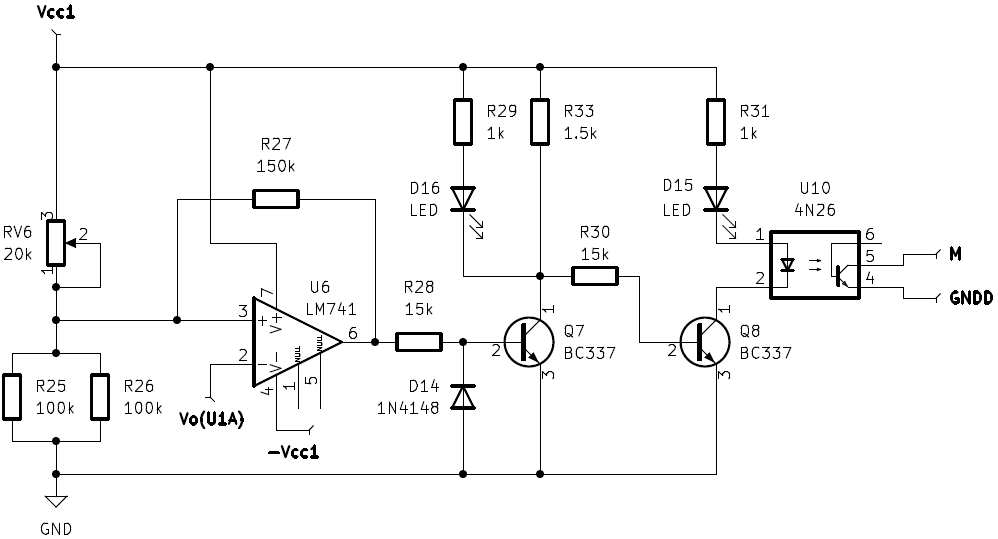
\includegraphics[width=0.9\textwidth]{./imagenes/modo_operacion.PNG}
    \caption{Sección de referencia de tensión.}
    \label{F:modo_operacion}
\end{figure}

\subsection{Integración del Circuito con NodeMCU ESP-32S}
Dado que no se requiere una conexión inalámbrica según las especificaciones del circuito, se ha prescindido del microcontrolador ESP con módulo Wi-Fi que tenía como objetivo la visualización de la información en un display, leer el estado de los \textit{encoders} rotativos y registrar los datos mas relevantes. Para mantener la aislación utilizaba el circuito integrado ISO1540 \cite{ISO1540}. El esquemático del circuito registrador que utilizaban puede observarse en la Figura \ref{F:ESP_32S}.
\begin{figure}[H]
    \centering
    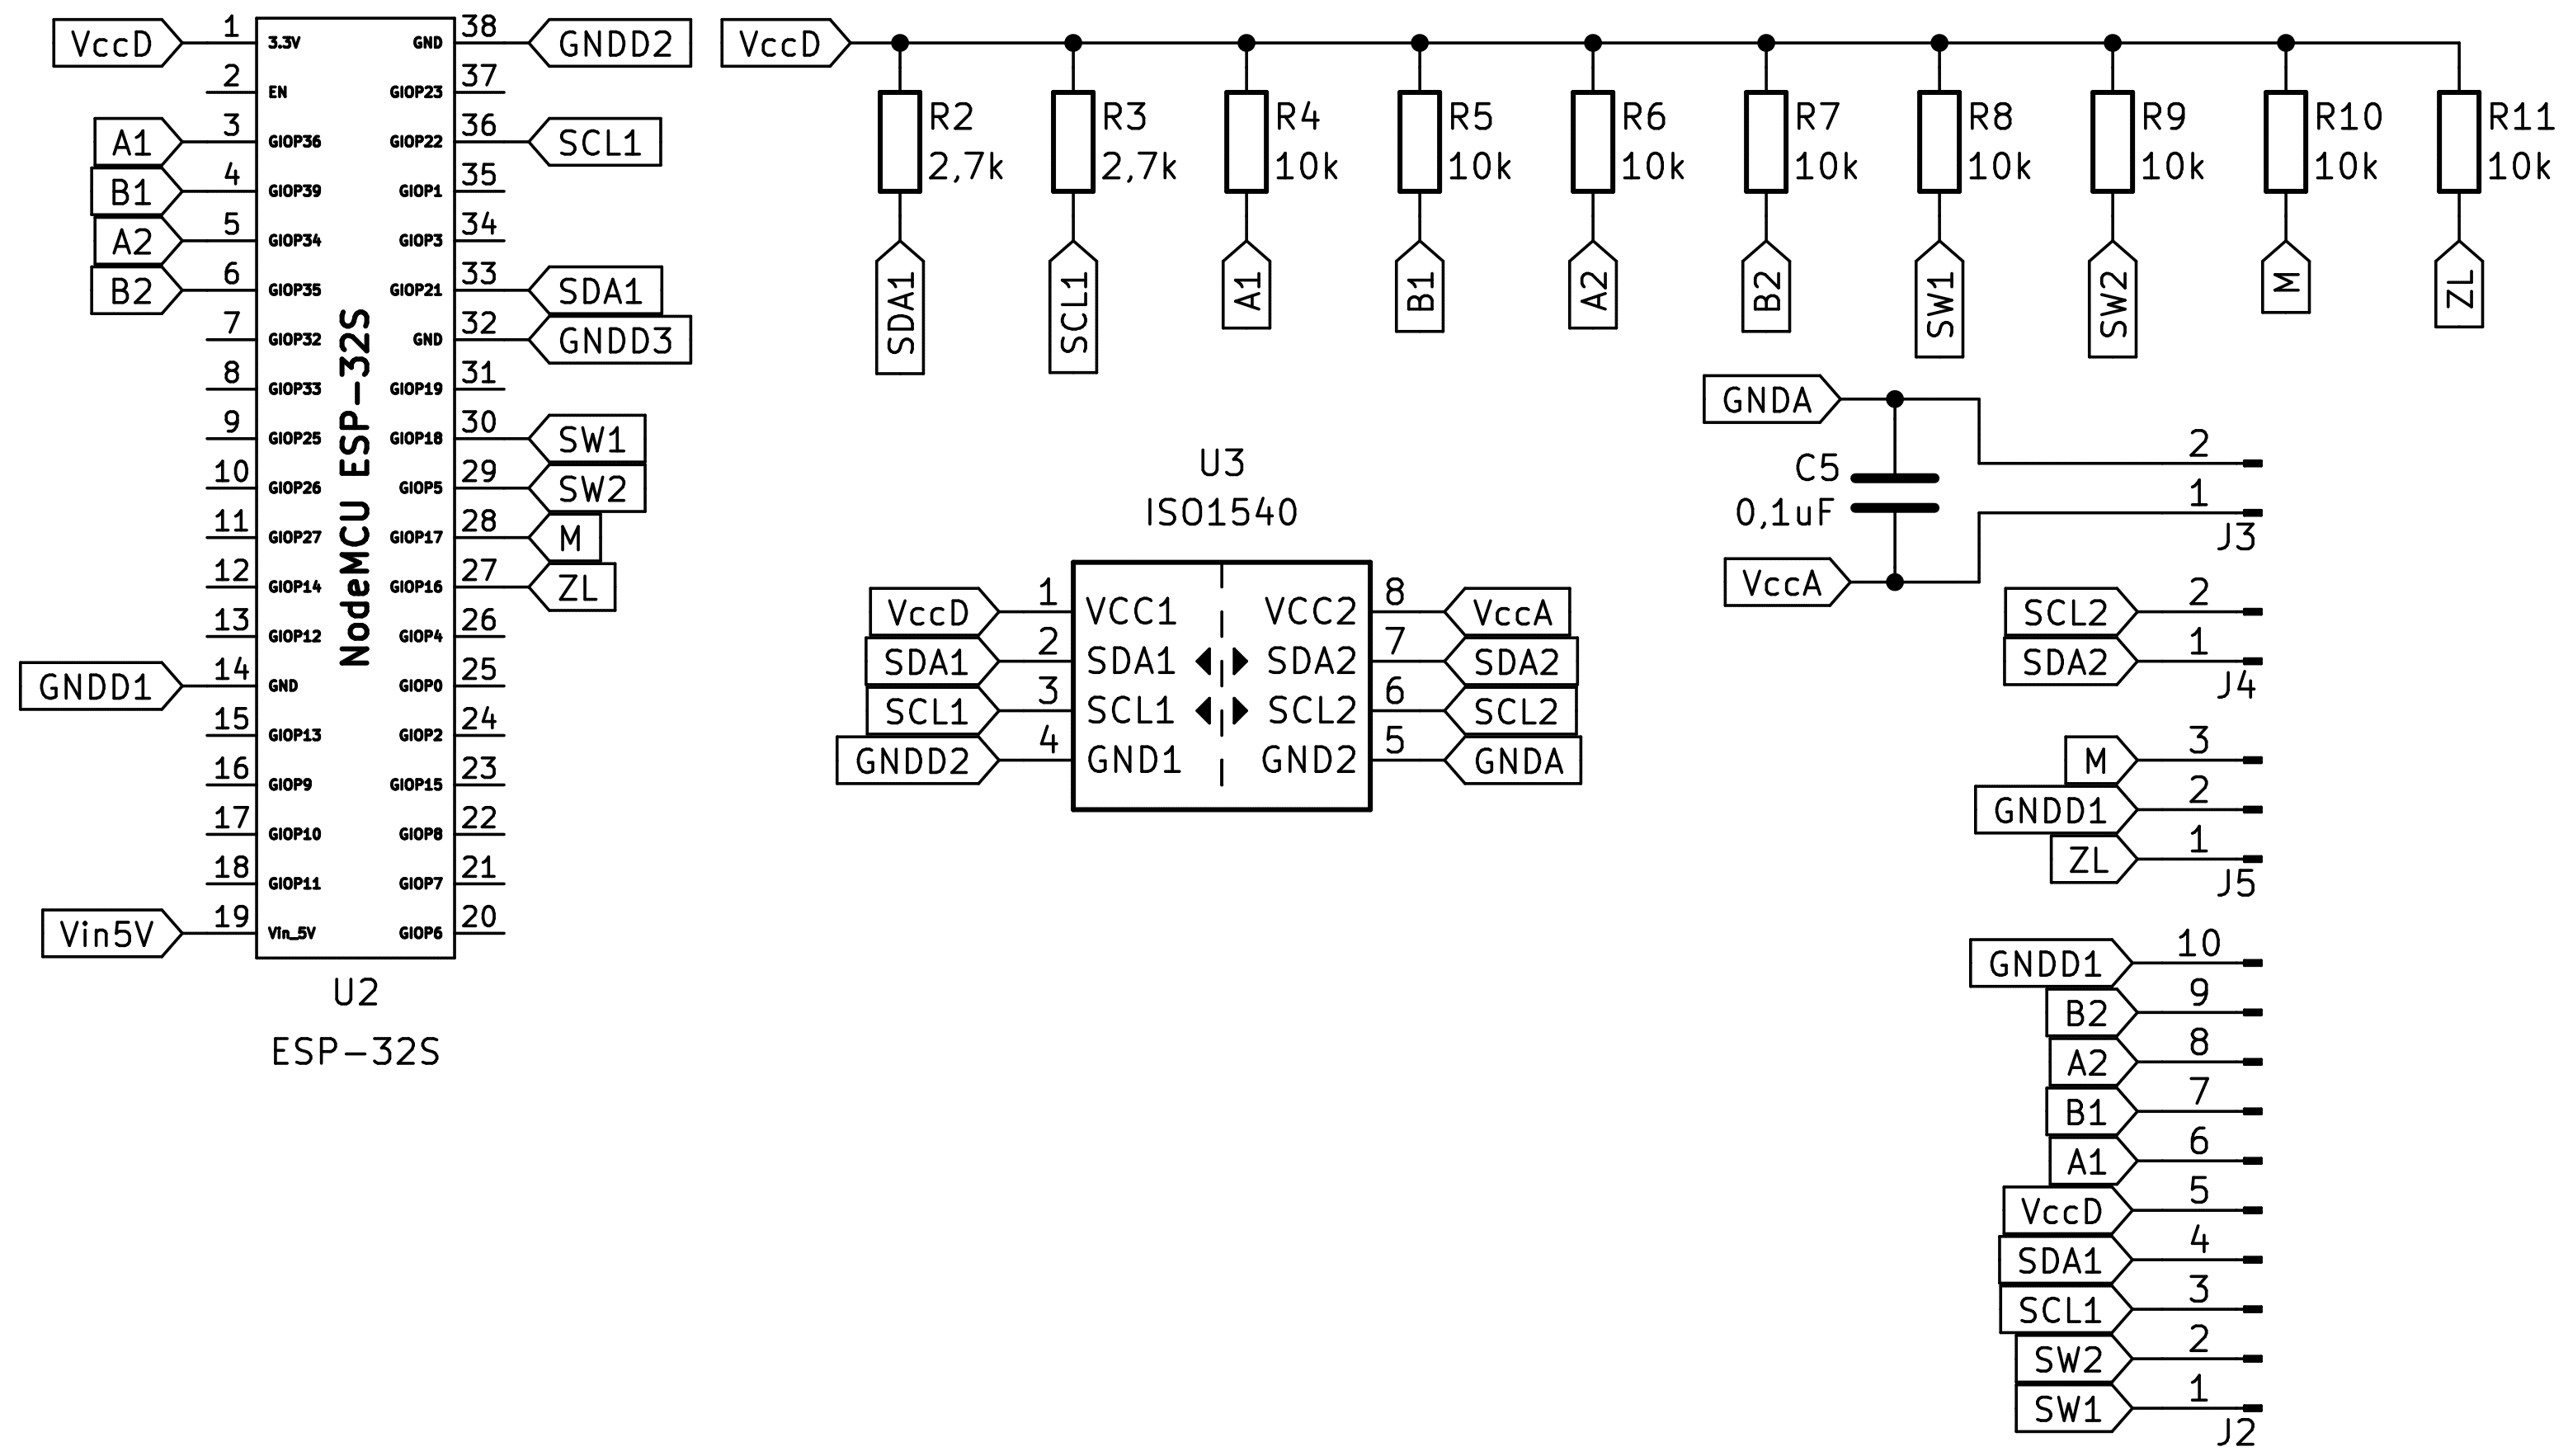
\includegraphics[width=0.8\textwidth]{./imagenes/ESP_32S.png}
    \caption{Circuito registrador de datos basado en el ESP-32S.}
    \label{F:ESP_32S}
\end{figure}

\subsection{Encoders rotativos}\par 
El uso de un teclado numérico hace que este elemento no sea necesario. Sin embargo, se dejará este elemento como una alternativa para el ajuste fino de las magnitudes a tiempo real. Esto se debe a una cuestión tradicional ya que la gran mayoría de los usuarios están acostumbrado a configurar manualmente las fuentes de tensión mediante perillas.\par
\begin{figure}[H]
    \centering
    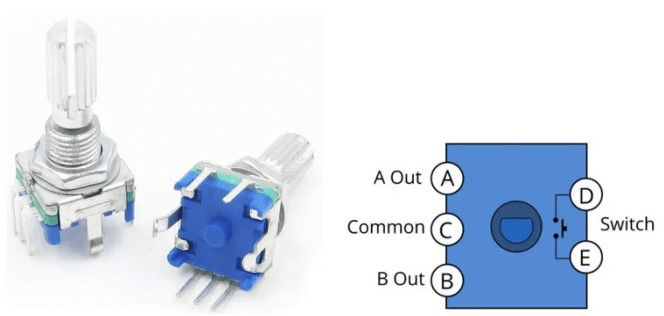
\includegraphics[scale=0.5]{./imagenes/encoder_rotativo.jpg}
    \caption{Encoder rotativo.}
    \label{F:encoder_rotativo}
\end{figure}
\par 
Estas modificaciones han permitido no solo modernizar la fuente de alimentación, sino también mejorar su funcionalidad y eficiencia mediante la incorporación de tecnología digital y la simplificación de circuitos redundantes. 

\section{Fuente de alimentación CC lineal planteada}

En la figura \ref{F:Diagrama_Bloques_general} se presenta el diagrama de bloques de la fuente de alimentación a diseñar. De la misma, la tensión de la red eléctrica alimentará a 3 transformadores: el principal de 33V eficaces para obtener la tensión a la salida, un secundario de (15+15)V con el fin de alimentar los circuitos en torno al punto de mayor tensión de la fuente y finalmente uno de 9V para alimentar la etapa digital.\par 
Los 33V del transformador principal serán rectificados y filtrados para obtener una tensión continua con un ripple reducido. Luego, ingresará al regulador con transistores BJT, los cuales trabajando en la zona activa permitirán el paso de la corriente hacia la salida. Para controlar estos últimos se empleará un conversor digital-analógico (DAC) para establecer un nivel de tensión sobre la base del arreglo de transistores. \par 
Para medir la tensión y la corriente se emplea unos circuitos acondicionadores de señal, con el fin de llevar las señales al rango de 0 a 5V empleado por el conversor analógico-digital (ADC). Para la medición de corriente se emplea una resistencia $R_{shunt}$ en serie con la salida. \par 
El circuito de acople y desacople de carga permite conectar y desconectar la carga en función del estado de la fuente. Esto permitirá proteger la carga ante condiciones de sobretensión o sobrecorriente.\par 
La parte digital se alimenta con una fuente de +5V obtenida a partir de la salida del transformador de 9V eficaces. El microcontrolador estará aislado completamente de la parte de potencia mediante un aislador I2C y optoacopladores según sea necesario. El programa que se ejecutará en el mismo buscará regular la tensión y corriente de salida de la fuente en función a los valores introducidos por el usuario. Para ello se podrá utilizar un teclado o perillas mientras que se visualizará los cambios en un display, constituyendo esta la interfaz entre la fuente y el usuario.

\begin{figure}[H]
    \centering
    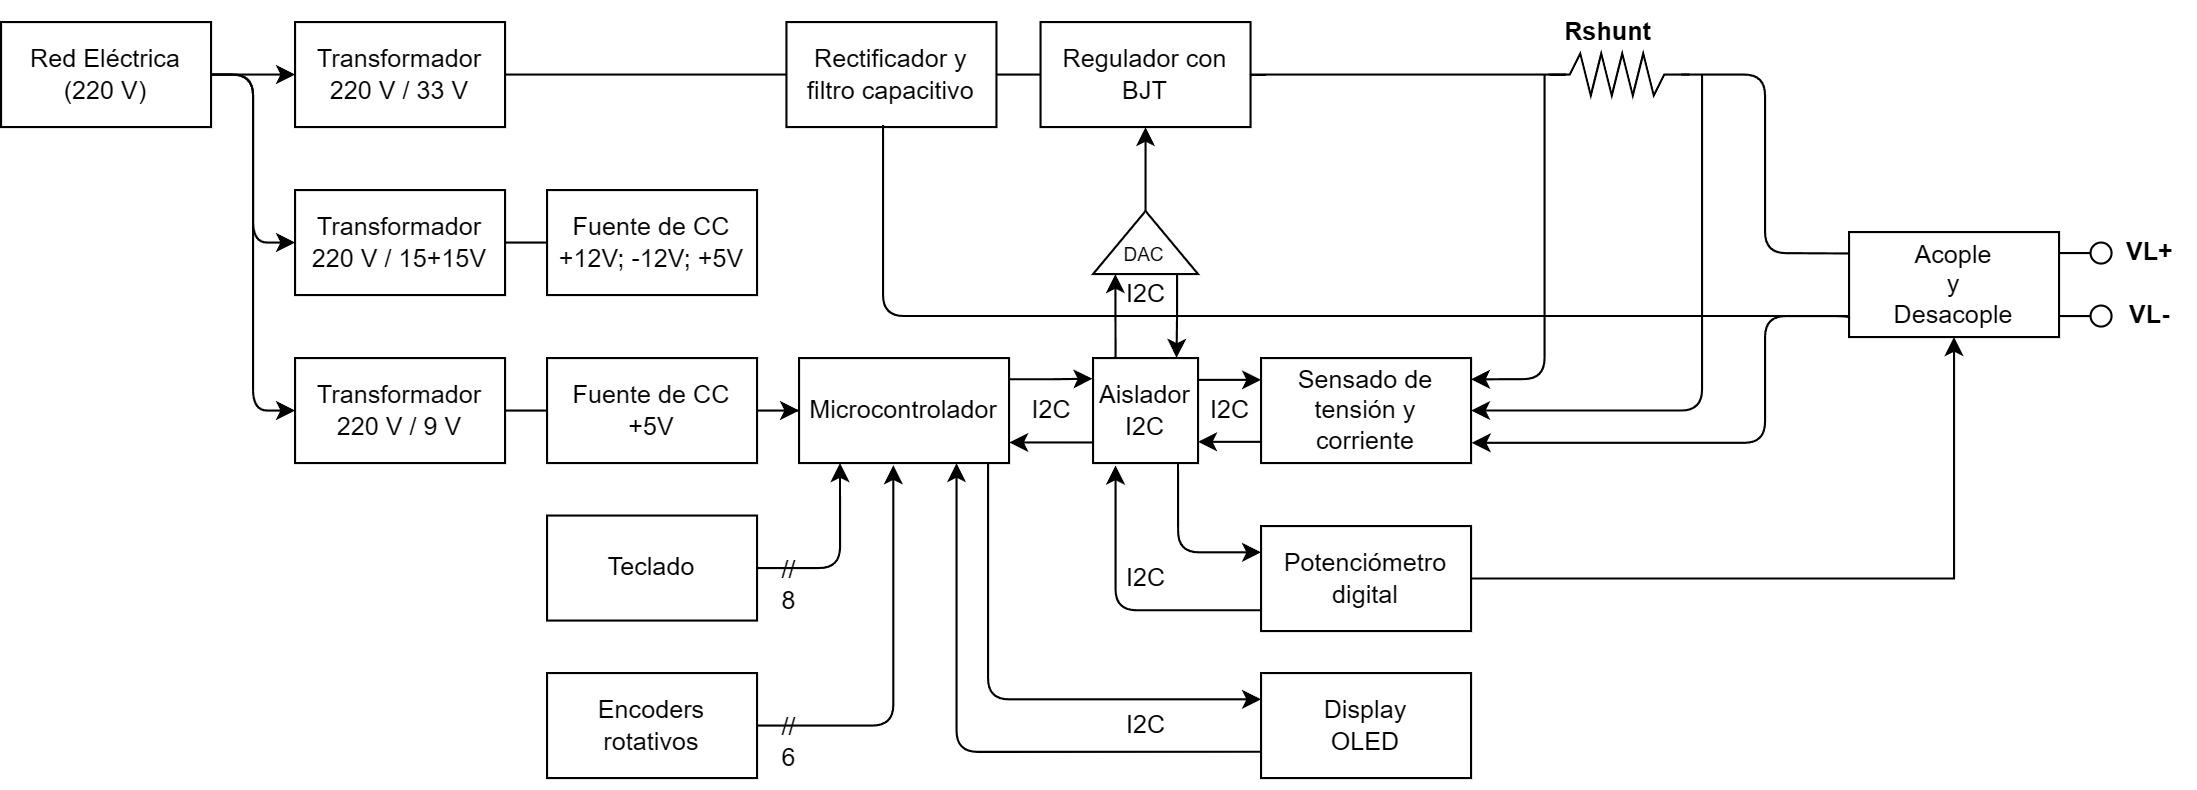
\includegraphics[width=\textwidth]{./imagenes/Diagrama_Bloques_general.jpg}
    \caption{Diagrama de bloques de la fuente de alimentación a diseñar}
    \label{F:Diagrama_Bloques_general}
\end{figure}


